\section{Literature Search}
\subsection{Multiply Accumulate}
The multiply accumulate (MAC) operation is perhaps the most important and fundamental operation in signal processing and deep learning.  It has the simple form:
$$ a \leftarrow a + (b\times c) $$
This operation is fundamental in signal processing because it easily describes feedback.  However it is even more important in general because it is the building block of matrix multiplication, which can be used to describe any finite linear transformation.  Two of the most computationally intense operations in deep learning for signal analysis are filtering (convolutional layer) and matrix multiplication (fully connected layer).  Since both operations are linear, one may think of a convolutional layer as a special case of a fully connected layer but having a special structure which makes its computation faster.

There are two primary architectures for high performance MAC computation: temproal and spatial. Temporal architectures use a central controller to aggregate the data of many arithmetic logic units (ALUs).  Spatial architectures allow direct communication between many ALUs in what is called ``dataflow processing.'' ~\cite{DBLP:journals/corr/SzeCYE17} 

\begin{figure}[H]
  \centering
  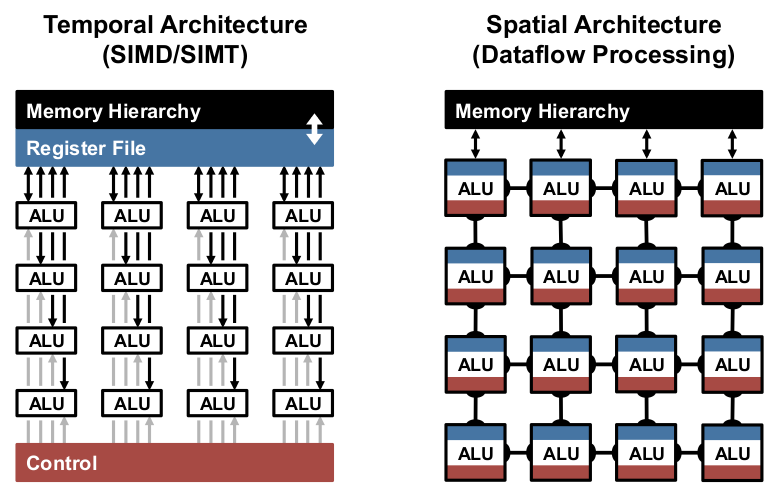
\includegraphics[width=10cm]{temporal_vs_spatial.png}
  \caption{Temporal and Spatial architectures  ~\cite{DBLP:journals/corr/SzeCYE17}}
\end{figure} 

\subsection{Optimization}
\subsubsection{Convolution}
A standard (finite) circular convolution can be computed using the ``flip and slide'' method [FF] with exactly $N_s N_f$ MACs where $N_s$ is the number of samples in the signal and $N_f$ is the number of filter coefficients.  However, it may be possible to do better.
The well known convolution theorem states that ``Convolution in the time (or spatial) domain is Hadamard (elementwise) multiplication in the frequency (temporal or spatial) domain.''  That is,
$$ x[n]\circledast y[n] = z[n] \implies X[k] \odot Y[k] = Z[k]$$
So we may calculate
$$ z[n] = \mathcal{F}^{-1}(\mathcal{F}(x[n]) \odot \mathcal{F}(y[n]))$$
It has been show that the lower bound on the number of multiplications for the fast fourier transform (for inputs of length $2^m$) is $ 4N - 2\log_2^2(N) - 2\log_2N - 4$, which has $O(N)$ complexity.  And in fact, there are known algorithms ~\cite{Winograd} which achieve this lower bound, but they use too many additions to be practical on modern processors. ~\cite{Duhamel:1990:FFT:78772.78773}  Practical algorithms such as the split-radix FFT achieve $4N\log_2{N} - 6N + 8$ real additions and multiplications, which is $O(N\log(N))$ complexity. ~\cite{Yavne:1968:EMC:1476589.1476610}  Additionally, when dealing with purely real data, there are algorithms which are capable of roughly halving the number of operations. ~\cite{Bergland:1968:NAF:364096.364118} Since our goal is to classify modulation using complex I-Q samples, it is unclear whether this optimization will be helpful, though previous work has suggested that complex neural networks offer only marginal imporvement. ~\cite{DBLP:journals/corr/TrabelsiBSSSMRB17}

It is clear that direct convolution computation has a complexity of $O(N_sN_f)$ while the Fourier transform method has a complexity of $O(N_s\log N_s)$, assuming that $N_f \leq N_s$ and we don't take advantage of the relative sparsity of the filter.  It is not immediately clear which of these is more practical.  If $N_s \rightarrow \infty$ as $N_f$ remains constant, the direct method is better.  If $N_s \rightarrow \infty$ and $N_f \rightarrow \infty$, the Fourier transform method is better.  We are also not accounting for the differing complexities and the fact that specialized hardware may exist for either.  Therefore experiment and deeper analysis will be necessary to determine which method is more suited to our application.


\subsubsection{Matrix Multiplication}




